\documentclass[12pt, letterpaper]{article}


\title{Optimizaci\'on no lineal \\  Tarea 1 }
\author{Natan Vilchis}

\date{6 de Agosto de 2018} 

\usepackage{hyperref}
\usepackage{amssymb}
\usepackage{graphicx}
\usepackage{apacite}
\usepackage{enumerate} 
\usepackage{commath}
\usepackage{amsmath}
\usepackage{booktabs}% http://ctan.org/pkg/booktabs
\usepackage{adjustbox}
\usepackage[spanish]{babel}
\usepackage[utf8]{inputenc}
\selectlanguage{spanish}
\decimalpoint

\usepackage{pythonhighlight}
\usepackage{listings} %For code in appendix
\lstset
{ %Formatting for code in appendix
    language=Python,
    basicstyle=\footnotesize,
    numbers=left,
    stepnumber=1,
    showstringspaces=false,
    tabsize=1,
    breaklines=true,
    breakatwhitespace=false,
}


\definecolor{gray97}{gray}{.97}
\definecolor{gray75}{gray}{.75}
\definecolor{gray45}{gray}{.45}

\graphicspath{ {images/} }

\hypersetup{
    colorlinks,
    citecolor=blue,
    filecolor=black,
    linkcolor=black,
    urlcolor=black
}

 
\begin{document}

\maketitle

\clearpage

\newcommand{\tabitem}{~~\llap{\textbullet}~~}
\renewcommand{\contentsname}{Tabla de contenido}
\renewcommand{\bibnodate}{s.f.}

\renewcommand{\refname}{Referencias}
\tableofcontents{} 
\clearpage



\section{Teor\'ia}
\subsection{Funcion continua}
Defina brevemente qu\'e es una funci\'on cont\'inua y d\'e un ejemplo de una funci\'on que cumpla la definici\'on y uno de una funci\'on que no la cumpla.

\subsubsection{Definici\'on }
Sea \textit{f}: A $\rightarrow$ $\mathbb{R}$ y \textit{a} $\in$ A. Se dice que \textit{f} es continua \cite{UniversityGranada} en \textit{a} cuando: 
\[ \forall \varepsilon \in \mathbb{R^+} \exists \delta \in \mathbb{R^+} \text{tal que} \mid x - \textit{a}\mid <  \delta  \Rightarrow \mid\textit{f}(x) - \textit{f}(\textit{a})\mid <  \varepsilon\] 

\subsubsection{Ejemplo de funci\'on continua}
Sea \textit{f}: $\mathbb{R}$ $\rightarrow$ $\mathbb{R}$ definida como sigue: f(x) = $x^2$ \\
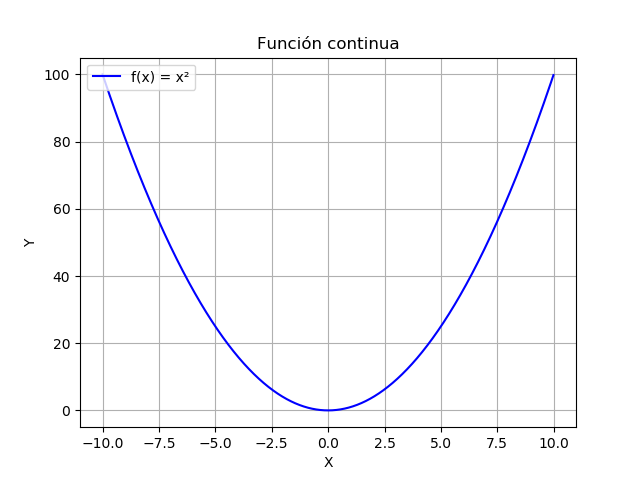
\includegraphics[scale=0.8]{funcontinous} \\ 
Veamos porqu\'e es continua \cite{Cimat}:\\
Sea $\varepsilon>0$ $\exists$ $\delta>0$ tal que si $|x-a|<\delta$ entonces $|x^2-a^2|<\varepsilon$.\\
Sin p\'erdida de generalidad podemos suponer que $\delta<1$. Por lo tanto, consideraremos valores de $x$ que satisfacen:\\
\begin{equation}\label{eq:demcontinuidad}
  0 < |x-a| <\delta \le  1 
\end{equation}\\
Usando (\ref{eq:demcontinuidad}) tenemos que:
\begin{align*}
|x^2-a^2|&=|(x-a)(x+a)| \\
		&\le|(x-a)(x-a+2a)| \\
			&\le |x-a|(|x-a|+2|a|)\\
			&\le |x-a|(1+2|a|)
\end{align*}
y queremos que esto sea menor que $\varepsilon$. Por lo tanto basta escoger $\delta$ que garantice que:
\[
  |x-a| < \frac{\varepsilon}{1+2|a|}
\]

Con:
\[
  \delta = min\{1,\frac{\varepsilon}{1+2|a|}\}
\]

\subsubsection{Ejemplo de funci\'on no continua}
Sea \textit{f}: $\mathbb{R}$ $\rightarrow$ $\mathbb{R}$ definida como sigue: \\
 \[
  f(x) = \left\{
     \begin{array}{@{}l@{\thinspace}l}
       \text{$2x+5$}  &,si \text{ $x\ge1$}\\
       \text{$2x-2$} &,si \text{ $x<1$}\\
    

     \end{array}
   \right.
\]

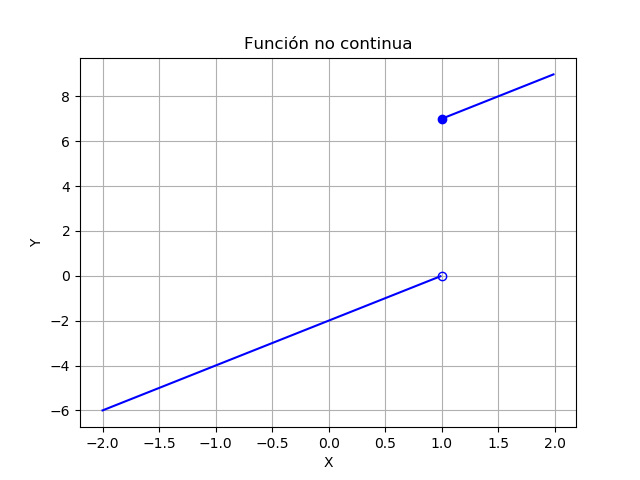
\includegraphics[scale=0.8]{funnotcontinous} \\
Notemos que en la gr\'afica tenemos un corte en la curva cuando $x=1$\\
Sea $\varepsilon=1$. Con $x<1$ y $|x-1|<\delta$\\
 \[
 |f(x)-f(1)|\ge |0-f(1)|=|f(1)|=|7|=7>1=\varepsilon
 \]
\subsection{Funci\'on diferenciable}	
Defina brevemente qu\'e es una funci\'on diferenciable y d\'e un ejemplo de una
funci\'on que cumpla la definici\'on y uno de una funci\'on que no la cumpla.
\subsubsection{Definici\'on}
Sea \cite{Cmat} \textit{f}: $\textbf{U}$ $\rightarrow$ $\mathbb{R}$, donde $\textbf{U}$ $\subset$ $\mathbb{R}^n$ es un conjunto abierto. La funci\'on f es diferenciable en un punto a $\in$ $\textbf{U}$, cuando existen n\'umeros reales $A_{1},\dots,A_{n}$ y una funci\'on $p$ definida en una bola $B(0, \varepsilon)$ con radio $\varepsilon >$  0, tal que, para todo $v$ = ($v_1$,$\dots$,$v_n$) $\in$  $\mathbb{R}^n$ con $a + v \in B(0,\varepsilon)$, se verifica:
\begin{equation}\label{eq:cond1diferenciable}
f(a+v) = f(a) + A_1 v_1 + \dots + A_n v_n +  \norm{v}p(v)
\end{equation}
\begin{equation}\label{eq:cond2diferenciable}
\lim_{x\to 0} p(v)= p(0)=0
\end{equation}

\subsubsection{Ejemplo de funci\'on diferenciable}
Sea \textit{f}: $\mathbb{R}$ $\rightarrow$ $\mathbb{R}$ definida como sigue: $f(x) = sin(x)$ \\
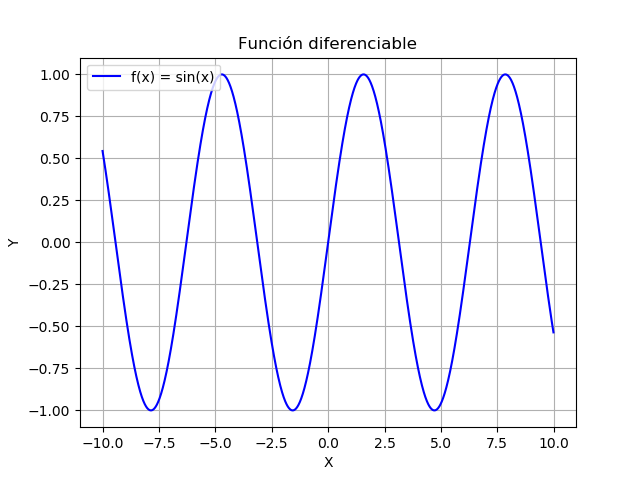
\includegraphics[scale=0.8]{diferenciable} \\


\subsubsection{Ejemplo de funci\'on no diferenciable}
Sea \textit{f}: $\mathbb{R}$ $\rightarrow$ $\mathbb{R}$ definida como sigue: $f(x) = |x|$ \\
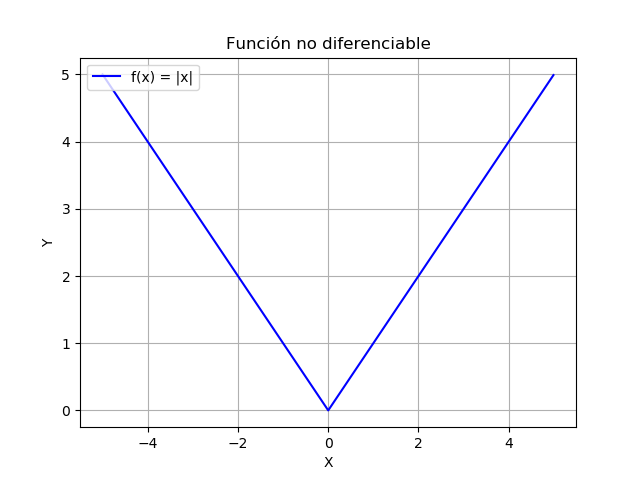
\includegraphics[scale=0.8]{notdiferenciable} \\
Esta funci\'on no es diferenciable en $x=0$.

\subsection{Funci\'on lineal}	
Defina brevemente qu\'e es una funci\'on lineal y mencione el tipo de fen\'omenos que \'estas modelan.
\subsubsection{Definici\'on}
Sea \textit{f}: $\mathbb{R}^n$ $\rightarrow$ $\mathbb{R}$ una función lineal definida como sigue: \\
\[f(x_1,x_2,\dots,x_n) = a_0 + a_1x_1+a_2x_2+\dots+a_nx_n \]\\


\subsubsection{Fenómenos que modelan}
Son fenómenos donde exista una conversión directamente proporcional para un problema, como el caso de dada temperatura en grados centígrados expresarla en grados K y verlo en una gráfica, o dado una ganancia de \$15 usd por hora ver la ganancia para x horas.
Por ejemplo:
\begin{enumerate}
\item Dado $x$ USD, podemos obtener su equivalencia en MXN (considerando el tipo de cambio al 9 de septiembre de 2018: $f_1(x)=18.72x$ 
\item Dado $x$ pulgadas, podemos obtener su equivalencia en centímetros: $f_2(x)=2.54x$ 
\item Dado $x$ K, podemos obtener su equivalencia en ºF: $f_3(x)=1.8x-459.67$ 
\end{enumerate}


\subsection{Funci\'on no lineal}
Defina brevemente una función no lineal y mencione el tipo de fenómenos que éstas modelan

\subsubsection{Definición}
Sea \textit{f}: $\mathbb{R}^n$ $\rightarrow$ $\mathbb{R}^n$ una función no lineal si la función no cumple con la definición de función lineal.
\subsubsection{Fenómenos que modelan}
Principalmente son fenómenos complejos donde intervienen varias variables y cambios con respecto a otras variables y que no puedan ser expresados mediante términos lineales, pudiendo ser cambios en la velocidad, aceleración, tiempo, de ciertas variables. Modelan fenómenos de la naturaleza como sismos, huracanes, transportes, entre otras cosas.
\subsubsection{Ejemplos}
\begin{enumerate}
\item $f_1(x)=x^2+35$
\item $f_2(x,y)=\log_{x}(x^2+y^2)$
\item $f_3(x,y,z,w)=x^2+35^y+x^{y^{z^{w^{w^{x^{y^{z}}}}}}}$
\end{enumerate}

\section{Programaci\'on}
\subsection{Lenguaje de programaci\'on \textit{compilado} y lenguaje de programaci\'on \textit{interpretado}}
Explique brevemente las diferencias, ventajas y desventajas entre un lenguaje de programaci\'on \textit{compilado} y un lenguaje de programaci\'on \textit{interpretado}.
\subsubsection{Diferencias, ventajas y desventajas}

La diferencia principal es el resultado de ejecutar las instrucciones del programa \cite{Indiana}. Un int\'erprete es un software capaz de producir un programa a partir de un lenguaje interpretado. Un compilador es un software capaz de producir un programa escrito en lenguaje ensamblador. 

\begin{tabular}{ l | p{5cm} |  p{5cm} c}
	\textbf{Concepto}   & \textbf{Lenguaje interpretado} & \textbf{Lenguaje compilado} \\
  \hline
	Diferencias & \tabitem BASIC, Java, Lisp,  Arc, Batch, Frontier, Groovy, Guile, Haskell, HyperCard, ICI, Icon, Io, Python, R, Ruby \cite{dmoztools_interpreted} son ejemplos de ellos.& \tabitem Ada, Algol 60, Assembly, Brainfuck, C--, C, C++, CHILL, Clipper, Cobol, Component Pascal, D, Modula-2 \cite{dmoztools_compiled} son ejemplos de ellos. \\
				& \tabitem El c\'odigo fuente es el programa  & \tabitem El compilado es ilegible.  \\
	                & \tabitem Mayor facilidad para aprender. & \tabitem El compilado es el programa. \\
	                & \tabitem Generalmente tipado din\'amico & \tabitem Generalmente tipado est\'atico. \\
\hline
	Ventajas & \tabitem F\'acil de depurar & \tabitem El compilado tiene mayor rapidez de ejecuci\'on.  \\
	          & \tabitem R\'apido desarrollo & \tabitem Permite crear un programa adecuado para cada plataforma \\
\hline
	Desventajas & \tabitem La ejecuci\'on del programa interpretado es m\'as lento & \tabitem S\'olo funciona en la plataforma para el que fue compilado. \\
	 &\tabitem Requiere del int\'erprete para funcionar& \tabitem Crear un programa compilado requiere varios pasos.\\
\end{tabular}


\subsubsection{Suma de matrices 10x10}
Genere con Octave dos matrices con entradas aleatorias, 10x10, y s\'umelas utilizando Octave, muestre en su reporte tanto las matrices generadas como la salida obtenida por el programa, con una captura de pantalla. \\ \\
Para la soluc\'on del programa de Matrices usaremos \textbf{Python3}, específicamente la versi\'on 3.7.0 \\\\
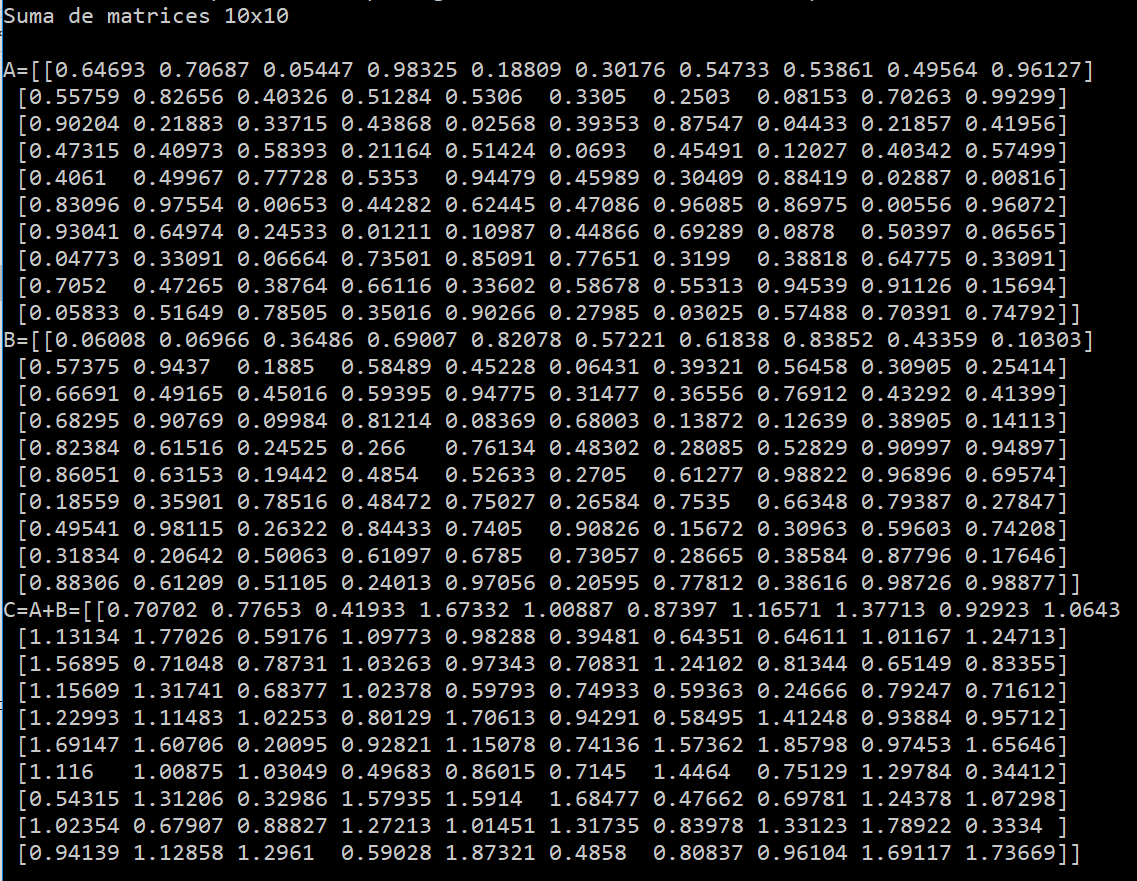
\includegraphics[scale=0.7]{matrices} \\

C\'odigo fuente:\\
\lstinputlisting[language=Python]{matrices.py}


\section{Investigaci\'on}

\subsection{Preguntas de optimizaci\'on}
Lea y Conteste detalladamente, y con sus propias palabras, a las siguientes
preguntas. Puede ayudarle leer el capítulo 1 de [?], o la introducción de
algún libro de optimización:\\
\begin{enumerate}[a)]  
\item \textbf{Describa de manera clara cu\'al es la importancia de la optimizaci\'on en la ingenier\'ia.}\\
Es importante debido a que los recursos que utiliza un determinado problema o trabajo son limitados. La optimización es importante debido a que es una herramienta capaz de lidiar con estos problemas al ofrecernos una solución que garantice que no hay otra solución mejor que la que hemos obtenido.
\item \textbf{¿Qu\'e elementos definen un problema de optimizaci\'on?}\\
Principalmente es la función objetivo, que incluye las variables del modelo a tratar y constantes. \\
Las variables del problema que representan algo en la vida real, como cantidad de personas para un trabajo, cantidad de computadoras, gasto energético, entre otras cosas.
También puede tener restricciones, que pueden ser por cada variable o bien una función o colección de funciones que hagan restricción a la función objetivo.

\item \textbf{¿C\'omo se clasifica un problema de optimizaci\'on?}\\
Como problema de optimización lineal o problema de optimización no lineal. También puede añadirse una subclasificación a cada uno de ellos si tratamos con valores enteros o reales. Así puede clasificarse en problema de optimización lineal entera o problema de optimización no lineal entera
\end{enumerate}
\subsection{Descripci\'on de dos aplicaciones a la vida real.}
Describa brevemente dos aplicaciones de la vida real, donde se requiera resolver un problema de optimización no lineal. Discuta la naturaleza no lineal de estos problemas.
\begin{enumerate}
\item El diseño de un elevador: Para este caso intervienen variables como el peso máximo que el elevador acepta, ajustar la velocidad para transportar el elevador con peso hacia arriba o hacia abajo, como se va a comportar en caso del freno de emergencia y que soporte el peso que se registra, o bien, en caso de un incidente añadir seguridad para que no caiga y afecte a las personas que se encuentran en el mismo.
\item El diseño de un carro:  Que sea aerodinámico, la forma de acomodar el motor, los asientos, los vidrios, pues al acomodarla de una forma va a ser más o menos aerodinámico, también el material con el que va a ser construido el chasis, la forma de éste para no sacrificar peso y quitar velocidad. La distancia de la llanta y su paralela, la altura que va a llevar el auto, la tracción en condiciones de lluvia, o incluso en nieve, la seguridad ABS, entre otras cosas. Esta aplicación es no lineal pues para cada problema que se describe tiene relación con todo y debe de ajustarse un óptimo diseño que considere todas esas variables.
\end{enumerate}

\subsection{Listado de las fuentes bibliogr\'aficas}
Liste aquí las fuentes bibliográficas, al menos una, a las que tendrá acceso en el curso. Indicar si cuenta con el libro por préstamo de la biblioteca, si lo tiene en formato electrónico, etc.\\
Cuento con ellos en formato electr\'onico (PDF): 
\begin{enumerate} 
\item Luenberger, D \&  Ye, Y. (2008). \textit{Linear and nonlinear Programming} Third Edition. USA:Springer 
\item Luenberger, D \&  Ye, Y. (2008). \textit{Linear and nonlinear Programming}  USA:Springer 
\item Taha, H. (2002)  \textit{Investigaci\'on de operaciones} Novena edici\'on.M\'exico: Pearson.
\item Hillier, F. \& Lieberman, G. (2006)  \textit{Introducci\'on a la investigaci\'on de operaciones} Octava edici\'on.M\'exico: McGraw-Hill/Interamericana Editores, S.A. de C.V. 
\item Luenberger, D. (1969)  \textit{Optimization by Vector Space Methods} USA: Wiley-Intersciene 
\item Barrera, P. (2012)  \textit{Introducci\'on a la optimización no lineal } M\'exico: Departamento de Matem\'aticas Universidad Aut\'onoma Metropolitana.
\item Ramos, A. (2012)  \textit{Optimizaci\'on no lineal } España: Universidad Pontifica Comillas.
\item \textit{Capítulo 2. Optimización no lineal} Archivo PDF. Colombia: Universidad Politécnica de Cartagena. Documento electrónico recuperado de:  \url{http://filemon.upct.es/~paredes/am_ti/apuntes/guia_onl.pdf}

\end{enumerate}
\clearpage
	
\bibliographystyle{apacite}
\bibliography{bibliography}
\end{document}
